\documentclass[11pt]{article}
\usepackage{icmlko}
\begin{document}

\title{한 도메인 안에서 부호가 뒤집히는 곳 --- 노트 79의 배제가 더 세게 확인됐다}
\author{월드모델 실험실}
\date{노트 372 · 2026년 8월 1일}
\maketitle

\begin{abstract}
노트 79가 만화에서 비일본 작품 583건을 뺐다. 근거는 ``KR 556건의 자기
순위 상관이 $+0.083$ 으로 일본 작품($+0.477$)의 6분의 1''이었고,
\textbf{그때 만화는 채점되지 않는 도메인이었다.} 노트 370이 만화를 유보
258행으로 채점 도메인으로 만들었으므로 \textbf{이제 유보에서 직접 갈라
볼 수 있다.} 학습은 JP 로 고정하고 유보만 풀어 한 번 적합 안에서
국가별로 쟀다.

\textbf{JP $+0.2567$(n=258, 같은 크기 무작위 대비 $p=0.000$) 대
KR $\mathbf{-0.1595}$(n=322, $p=1.000$).} 약한 것이 아니라
\textbf{뒤집혀 있다} --- 일본 만화로 배운 모형이 한국 웹툰에서는 순서를
거꾸로 매긴다. 셋을 섞으면 $+0.0563$ 으로 무작위와 같아진다.
연도를 맞춰도 갈린다(KR 2025 $-0.2016$, n=279). 그리고 \textbf{라벨
중앙이 JP 3.05 · KR 3.10 으로 거의 같다} --- 노트 353(연도 사이 수준) ·
357(계수 기준 수준)과 달리 \textbf{수준이 아니라 부호}다.
\textbf{노트 79의 배제는 지금 판에서 더 세게 선다.} 만화 유보는 258행에
머문다.
\end{abstract}

\section{이제는 직접 갈라 볼 수 있다}

노트 79의 근거는 \emph{자기 순위 상관}이었다 --- 만화가 채점 도메인이
아니었으니 그것밖에 못 쟀다. 노트 370 이후로는 유보가 있다. 학습을
JP 1,783행으로 고정하고 유보만 풀어(JP 258 · KR 322 · CN 19) \textbf{한
번의 적합 안에서} 부분집합끼리 견줬다 --- 노트 371이 그은 경계
(``짝이냐가 아니라 같은 실험 안이냐'')를 지키는 읽기다.

\begin{center}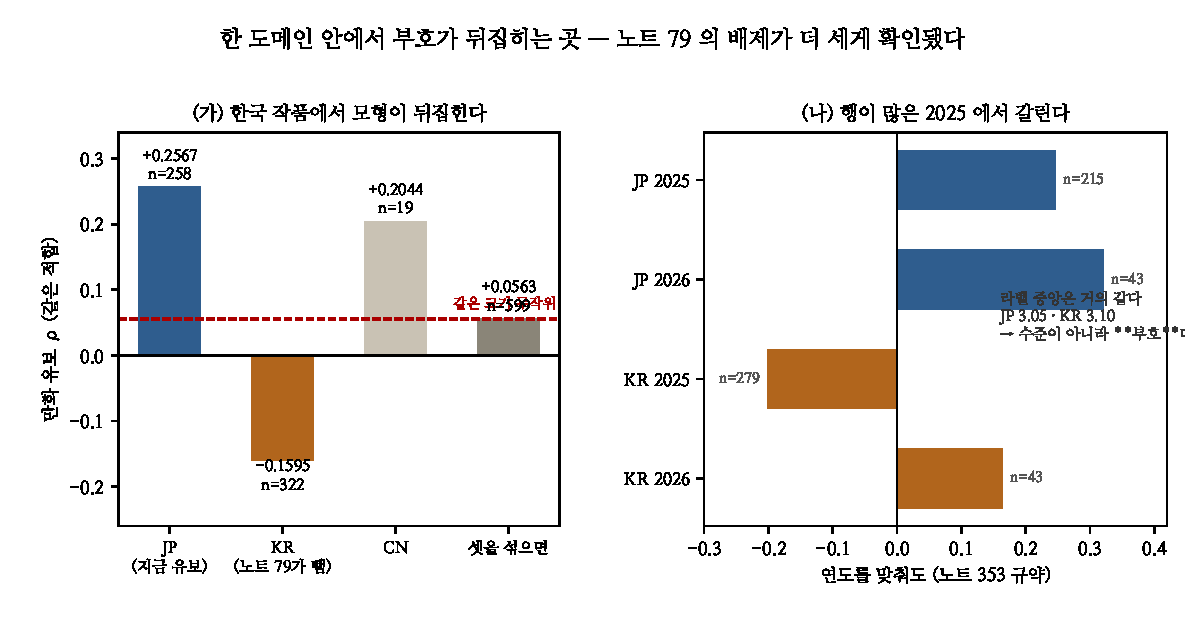
\includegraphics[width=\linewidth]{figs/inv.pdf}\end{center}

\begin{center}
\begin{tabular}{lrrl}
\hline
국가 & $n$ & $\rho$ & 같은 크기 무작위 \\
\hline
JP & 258 & $\mathbf{+0.2567}$ & $+0.0546$ (SD 0.047) $p=0.000$ \\
KR & 322 & $\mathbf{-0.1595}$ & $+0.0555$ (SD 0.036) $p=1.000$ \\
CN & 19 & $+0.2044$ & (작아서 못 가름) \\
\hline
셋을 섞으면 & 599 & $+0.0563$ & --- \\
\hline
\end{tabular}
\end{center}

\textbf{KR 은 약한 것이 아니라 음수다.} 같은 크기 무작위 부분집합보다
나쁘고($p=1.000$), 섞으면 만화 전체가 $+0.0563$ 으로 무작위 수준이 된다.

\section{수준이 아니라 부호다}

이 창에서 ``두 모집단이 안 섞인다''를 세 번 만났다. 앞의 둘과 여기가
다르다.

\begin{center}
\begin{tabular}{lll}
\hline
 & 무엇이 달랐나 & 어떻게 알았나 \\
\hline
노트 353 아이돌 & 연도 사이 \textbf{수준} & 라벨 중앙 $-0.61$ 대 $+0.49$ \\
노트 357 팝업 & 계수 기준 \textbf{수준} & 주장이 해마다 $+0.27\!\sim\!+0.44$ 높다 \\
\textbf{노트 372 만화} & \textbf{부호} & 라벨 중앙 3.05 대 3.10 --- \emph{같다} \\
\hline
\end{tabular}
\end{center}

앞의 둘은 곱셈 부풀림이라 \emph{섞을 때만} 해로웠다(기준 안에서는
멀쩡했다). 여기는 KR 만 따로 재도 음수다 --- \textbf{축과 라벨의 관계
자체가 반대로 서 있다.}

\textbf{까닭은 노트 79가 적어 둔 그대로다.} 라벨이 \emph{세계 독자}의
서재 등록 수이고, 한국 작품에서는 그것이 영어 번역 유무에 지배되는데
AniList 메타데이터가 그것을 안 담는다. 우리 축이 보는 것(연재 밀도 ·
작가 사전 작품 · 태그 폭)은 일본 시장에서는 순서를 만들고 한국 작품에서는
\emph{번역 여부와 반대로} 걸린다 --- 오래 연재된 인기 웹툰일수록 축은
높게 보는데 AniList 등록 수는 영어권 진출 여부로 갈린다.

\textbf{연도를 맞춰도 남는다}(노트 353 규약): KR 2025 $-0.2016$(n=279) ·
KR 2026 $+0.1636$(n=43). 행이 많은 2025 에서 음수다.

\section{그래서 안 넣는다}

만화 유보는 258행에 머문다. 583행을 더 넣으면 만화가 $0.2520 \to 0.0563$
으로 무너지고 판이 그만큼 내려간다 --- \emph{측정력이 느는 게 아니라
과제가 망가진다.}

\textbf{노트 79는 여섯 해 전 판에서 옳았고 지금 판에서 더 옳다.} 노트
361이 ``남은 것 표의 수는 인용할 때마다 다시 잰다''고 적었는데, 다시 재니
\emph{같은 결론이 더 센 증거로} 나왔다. \textbf{다시 재는 것은 뒤집기
위해서가 아니다.}

\section{규약에 더하는 줄}

\begin{itemize}
\item \textbf{``안 섞인다''에는 두 종류가 있다} --- \emph{수준}이 다른
것(353 · 357)과 \emph{부호}가 다른 것(372). 앞은 기준 안에서 멀쩡하니
따로 재면 쓸 수 있고, 뒤는 따로 재도 못 쓴다. \textbf{둘을 가르려면
부분집합을 따로 채점해 본다.}
\item \textbf{도메인 안 부분모집단은 유보가 생긴 뒤에 다시 잰다.} 채점이
안 되던 시절의 근거(자기 상관)는 약한 대리다.
\end{itemize}

\section{남은 것}

\begin{center}
\begin{tabular}{ll}
\hline
갈래 & 지금 아는 것 \\
\hline
세계애니 눈금 & 합친 백분위가 세계애니를 12/12 로 올렸다(노트 369) \\
팝업 실측 41행 & 노트 360 · 364 · 366 \\
KR 웹툰을 웹툰 도메인으로 & AniList KR 322건은 시장이 웹툰과 같다. \\
 & 라벨(세계 서재 등록)만 다르다 --- 붙일 자리가 있나 \\
\hline
\end{tabular}
\end{center}

마지막 줄이 이 노트가 연 것이다. KR 작품이 만화에서 못 쓰이는 이유가
\emph{라벨}이라면, 같은 작품을 네이버 즐겨찾기로 재는 웹툰 도메인에서는
멀쩡할 수 있다. 다만 노트 365의 제목 대조에서 정규화 일치가 0\%였다
(로마자 표기) --- 붙이려면 제목 정합부터다.

\end{document}
